\chapter{Tensor Algebra, Metrics, and the First Step to Space-Time}

This lecture marks a threshold in the course. Susskind says again that he is after the ``theoretical minimum,'' but now adds an important warning: if one were merely to announce the answers in words, that would be less than the minimum. From this point on, the minimum already requires patient calculation. We therefore follow the lecture's progression closely. We begin with transformation laws, not pictures; we build tensor algebra from those laws; we introduce the metric as the first genuinely geometric tensor in the story; and only then do we pivot to flat space, special relativity, and a first time-dependent cosmological metric. These companion notes follow Leonard Susskind's lecture closely and preserve selected documentary board frames associated with LazyingArt LLC and Video2Book.

\section{Covariant and Contravariant Review}

Susskind begins by slowing the room down. We are to review the transformation properties of covariant and contravariant components before trying to do anything more difficult. The reason is not bureaucratic. In curved geometry, and later in space-time, everything depends on knowing exactly what kind of object one is dealing with.

Let \(x^m\) and \(y^m\) denote two coordinate systems. The convention in the lecture is that coordinates themselves carry upper indices. Once that choice is made, the transformation rules are easy to read.

A covariant object transforms as
\begin{equation}
V_m(y)=\frac{\partial x^n}{\partial y^m}V_n(x),
\end{equation}
while a contravariant object transforms as
\begin{equation}
W^m(y)=\frac{\partial y^m}{\partial x^n}W^n(x).
\end{equation}

This is the point at which Susskind insists that a vector is not ``any three numbers'' or ``anything that can be drawn as an arrow.'' Temperature, pressure, and humidity give three numbers, but they do not transform as components of a vector. They are just three scalars placed side by side. A vector is defined by its transformation law.

The two basic archetypes come straight from multivariable calculus. If \(\phi\) is a scalar field, then
\begin{equation}
\frac{\partial \phi}{\partial y^m}
=
\frac{\partial \phi}{\partial x^n}
\frac{\partial x^n}{\partial y^m},
\end{equation}
so the gradient transforms covariantly. And if \(y^m=y^m(x)\), then
\begin{equation}
dy^m=\frac{\partial y^m}{\partial x^n}\,dx^n,
\end{equation}
so a differential displacement transforms contravariantly. These are not postulates invented to make tensor calculus elegant. They are chain rules.

It is worth preserving another small but useful convention from the lecture: once the coordinates are written with upper indices, it becomes difficult to get lost. A derivative \(\partial x^n/\partial y^m\) naturally carries one upper \(n\) and one lower \(m\), and those index positions tell us which kind of object it is prepared to convert into which other kind.

\subsection{Question \& Answer}

\paragraph{Question.} If an object satisfies one of the vector transformation laws, must it satisfy the other one too?

\paragraph{Answer.} Not yet. The lecture is careful about this. At first, a covariant vector and a contravariant vector are simply different kinds of objects. A gradient,
\[
\frac{\partial \phi}{\partial x^m},
\]
is covariant. A small displacement,
\[
dx^m,
\]
is contravariant. We are not yet entitled to identify them as two forms of the same vector. That identification only becomes natural once the metric has been introduced and we learn how to raise and lower indices.

\section{From Vectors to General Tensors}

Once we understand the one-index case, the multi-index case is almost forced on us. Each index transforms, and each index brings its own Jacobian factor. For a rank-two covariant tensor,
\begin{equation}
T_{mr}(y)=
\frac{\partial x^n}{\partial y^m}
\frac{\partial x^s}{\partial y^r}
T_{ns}(x).
\end{equation}
For a mixed tensor with one upper and one lower index,
\begin{equation}
T^m{}_{n}(y)=
\frac{\partial y^m}{\partial x^s}
\frac{\partial x^r}{\partial y^n}
T^s{}_{r}(x).
\end{equation}

This is the general pattern Susskind wants us to absorb. Indices are not decoration. They are instructions for transformation.

He then turns to the next basic operation, contraction. If one upper and one lower index are identified and summed over, the rank drops. For example,
\begin{equation}
T^m{}_{m}=T^1{}_{1}+T^2{}_{2}+T^3{}_{3}+\cdots.
\end{equation}
No free index remains, so one expects a scalar. The lecture then checks it explicitly.

If we transform \(T^m{}_{n}\) and then set the two indices equal, the Jacobian factors combine to
\begin{equation}
\frac{\partial x^r}{\partial y^m}
\frac{\partial y^m}{\partial x^s}
=
\delta^r{}_{s}.
\end{equation}
This is the Kronecker delta, the identity tensor, with one upper and one lower index. It tells us to set \(r=s\). Therefore
\begin{equation}
T^m{}_{m}(y)=T^r{}_{r}(x),
\end{equation}
and the contracted quantity is indeed a scalar.

The same operation works more generally. If we start with a tensor carrying many upper and lower indices, identify one upper with one lower, and sum, the result is a tensor of lower rank. This is one of the main engines of tensor algebra.

A familiar special case is the inner product. If \(v^m\) is contravariant and \(w_m\) is covariant, then
\begin{equation}
v^m w_m
\end{equation}
is a scalar.

\subsection{Question \& Answer}

\paragraph{Question.} If we contract one index of a higher-rank tensor, does that mean the original tensor was simply a scalar times a smaller tensor?

\paragraph{Answer.} No. The lecture pauses on exactly this point. Contraction is an operation that produces a new tensor of lower rank. In special cases the new object may factor in a simple way, but in general it does not mean the original tensor was merely a scalar multiple of some simpler one. The contraction throws away structure; it does not reveal a hidden trivial factorization.

This is why contraction matters. It is not just notation. It manufactures coordinate-independent quantities and lower-rank tensors from more complicated ones.

\section{The Metric Tensor as Distance}

At this point the lecture turns from pure index bookkeeping to the first tensor with direct geometric meaning: the metric tensor. If two neighboring points are separated by the infinitesimal displacement \(dx^m\), then the squared distance between them is
\begin{equation}
ds^2=g_{mn}(x)\,dx^m dx^n.
\end{equation}

The form of this expression is already telling. The two \(dx\)'s contribute two contravariant indices; the metric contributes two covariant ones; everything is contracted; no free indices remain. Thus \(ds^2\) is a scalar.

Now comes the decisive question: is \(g_{mn}\) really a tensor? Susskind does not answer by appeal to intuition. He answers by rewriting the same interval in another coordinate system.

We have
\begin{equation}
dx^m=\frac{\partial x^m}{\partial y^r}\,dy^r.
\end{equation}
Substituting twice into the line element gives
\begin{align}
ds^2
&=
g_{mn}(x)\,dx^m dx^n \\
&=
g_{mn}(x)
\frac{\partial x^m}{\partial y^r}
\frac{\partial x^n}{\partial y^s}
dy^r dy^s.
\end{align}
Now define the coefficient of \(dy^r dy^s\) to be the metric in the \(y\)-coordinates:
\begin{equation}
g_{rs}(y)=
\frac{\partial x^m}{\partial y^r}
\frac{\partial x^n}{\partial y^s}
g_{mn}(x).
\end{equation}
But this is exactly the transformation law for a covariant rank-two tensor. The metric is therefore a tensor in the strict sense used throughout the lecture.

\paragraph{Worked derivation.} The derivation is short enough to summarize in the same clipped order in which the lecture presents it:
\begin{enumerate}
\item Write the squared distance as \(ds^2=g_{mn}(x)\,dx^m dx^n\).
\item Rewrite each \(dx^m\) in terms of \(dy^r\).
\item Substitute and collect the coefficient of \(dy^r dy^s\).
\item Call that coefficient \(g_{rs}(y)\).
\item Read off the tensor transformation law.
\end{enumerate}

The lecture is careful about what this proves. It proves that the same scalar interval may be expressed in different coordinates using metric components related by the tensor law. It does not mean that two unrelated formulas happen to agree.

\subsection{Question \& Answer}

\paragraph{Question.} Is \(ds^2\) ``the same regardless of the coordinates''?

\paragraph{Answer.} Yes, but only in the precise sense just described. We are not computing two different distances and discovering a coincidence. We are taking one and the same scalar interval and rewriting it. That rewriting forces the relation between \(g_{mn}(x)\) and \(g_{rs}(y)\). The invariance of \(ds^2\) is therefore not a separate afterthought; it is the starting point of the metric transformation law.

\section{Metric as Matrix, Inverse Metric, and Raising/Lowering}

Once the metric has been established as a tensor, the lecture immediately shifts register. A rank-two tensor, viewed at a fixed point and in a fixed coordinate system, is also a matrix. Strictly speaking the tensor is not the matrix; rather, its components in a given coordinate system form a matrix. But Susskind moves freely between those two descriptions, and the notes should do the same.

\begin{figure}[htbp]
\centering

\includegraphics[width=0.78\textwidth]{lecture_04_figure_04.png}
\caption{Metric tensor as matrix and inverse}
\end{figure}

Thus we may write
\begin{equation}
g_{mn}\leftrightarrow
\begin{pmatrix}
g_{11} & g_{12} & g_{13} & \cdots \\
g_{21} & g_{22} & g_{23} & \cdots \\
g_{31} & g_{32} & g_{33} & \cdots \\
\vdots & \vdots & \vdots & \ddots
\end{pmatrix}.
\end{equation}
For the line element, the lecture takes the metric to be symmetric,
\[
g_{mn}=g_{nm},
\]
and then introduces its inverse as an ordinary matrix inverse.

At the matrix level one writes
\begin{equation}
g^{-1}g=I.
\end{equation}
In index notation that becomes
\begin{equation}
g^{mr}g_{rn}=\delta^m{}_{n}.
\end{equation}
Here the Kronecker delta must carry one upper and one lower index. The lecture explicitly stops to correct the temptation to write both indices downstairs. In tensor notation \(\delta^m{}_{n}\) is the identity tensor.

\begin{figure}[htbp]
\centering

\includegraphics[width=0.72\textwidth]{lecture_04_figure_02.png}
\caption{Inverse metric contraction identity}
\end{figure}

The upper-index object \(g^{mn}\) is then interpreted as the collection of components of the inverse matrix. This is not a new geometric structure carrying new information; it is another representation of the same metric. The nontrivial theorem, stated but not proved in the lecture, is that these inverse-matrix components themselves transform tensorially, now as a contravariant rank-two tensor.

It is therefore legitimate to speak of the metric with lower indices and the metric with upper indices. They contain the same information.

The lecture also gives a simple worked example. In polar coordinates on the plane,
\begin{equation}
ds^2=dr^2+r^2 d\theta^2.
\end{equation}
If \(r\) is the first coordinate and \(\theta\) the second, then
\begin{equation}
g_{11}=1,\qquad g_{22}=r^2,
\end{equation}
with no off-diagonal terms. The inverse metric is therefore
\begin{equation}
g^{11}=1,\qquad g^{22}=\frac{1}{r^2}.
\end{equation}
For a diagonal matrix, the inverse is found by inverting the diagonal entries.

\subsection{Question \& Answer}

\paragraph{Question.} Can the metric tensor fail to have an inverse?

\paragraph{Answer.} A general tensor can fail to have an inverse, but the lecture insists that the metric is not of that kind. Susskind attributes this to symmetry together with the absence of zero eigenvalues, and then postpones the proof. For the purposes of the lecture, invertibility is part of the working definition of the metric structure we are using.

\begin{figure}[htbp]
\centering

\includegraphics[width=0.72\textwidth]{lecture_04_figure_03.png}
\caption{Inverse metric relation}
\end{figure}

\subsection{Question \& Answer}

\paragraph{Question.} Why may we take the metric to be symmetric?

\paragraph{Answer.} Because only the symmetric part contributes to the quadratic form \(ds^2\). The cross terms appear as
\begin{equation}
g_{12}\,dx^1 dx^2+g_{21}\,dx^2 dx^1
=
(g_{12}+g_{21})\,dx^1 dx^2,
\end{equation}
since \(dx^1dx^2=dx^2dx^1\). The antisymmetric part cancels out of the line element. There is therefore no loss of generality, for the purposes of distance, in taking the metric symmetric.

Now comes the first serious use of the metric. Given contravariant components \(V^m\), we define the corresponding covariant components by
\begin{equation}
V_n=g_{nm}V^m.
\end{equation}
Conversely,
\begin{equation}
V^m=g^{mn}V_n.
\end{equation}
Likewise, for a rank-two tensor,
\begin{equation}
T^m{}_{n}=g^{mr}T_{rn}.
\end{equation}
This is the operation of raising and lowering indices.

The lecture then applies the same idea to the differential displacement:
\begin{equation}
dx_m=g_{mn}\,dx^n.
\end{equation}

\begin{figure}[htbp]
\centering

\includegraphics[width=0.76\textwidth]{lecture_04_figure_05.png}
\caption{Lowering an index with the metric}
\end{figure}

The board at this stage is pedagogically valuable because the circled factor marks the lowering step. It is also slightly misleading: the first chalk line suggests a literal equality that Susskind later withdraws. What is intended is a contraction step, not an equality between unlike expressions. Written cleanly, the argument is
\begin{align}
dx^m dx_m
&=
dx^m\bigl(g_{mn}dx^n\bigr) \\
&=
g_{mn}\,dx^m dx^n \\
&=
ds^2.
\end{align}
There is also a third equivalent form:
\begin{equation}
g^{mn}dx_m dx_n=ds^2.
\end{equation}
So the same scalar interval may be written in three ways:
\begin{equation}
ds^2=g_{mn}\,dx^m dx^n=dx^m dx_m=g^{mn}dx_m dx_n.
\end{equation}

This is the moment at which the early separation between covariant and contravariant components softens. Once the metric is given, the lecture is perfectly willing to speak of upper and lower components of the same vector.

\section{Tensor Equalities and the End of Tensor Algebra}

Having developed the metric and its inverse, the lecture briefly returns to the general algebra of tensors and extracts two useful principles.

The first is a warning. Tensors may be added only if they are of the same type. It makes sense to add \(T_{mn}\) and \(W_{mn}\). It does not make sense to add, say, a tensor with lower indices to one with upper indices and expect the result to transform coherently. The index structure is part of the identity of the tensor.

The second principle is much more powerful. If a tensor is zero in one coordinate system, it is zero in every coordinate system. The reason is immediate from the transformation law: the transformed components are Jacobian factors multiplying the original components. If the original components are zero, the transformed components are zero.

From this it follows that if two tensors are equal in one coordinate system, they are equal in every coordinate system. Indeed, if
\[
T=W
\]
in one coordinate system, then
\[
T-W=0
\]
there; but a zero tensor is zero everywhere, so \(T=W\) everywhere.

This is why tensor equations are so powerful. Each side may have complicated coordinate dependence in its separate components, but if the two sides are equal once, they remain equal after every legitimate coordinate transformation. The equality is geometric, not coordinate-bound.

At this point the lecture gestures toward tensor calculus and then refuses to begin it. Ordinary derivatives of tensor components are not, in general, tensor components. One needs a more careful notion of differentiation. Susskind postpones that subject to the next lecture, and the postponement is deliberate. He wants the class to leave tensor algebra with a clean pivot into space-time.

\section{Flat Space, Cartesian Frames, and the Pivot to Space-Time}

The re-entry into geometry is through the simplest case: ordinary flat space. Even if we restrict ourselves entirely to Cartesian coordinates, there is still more than one Cartesian coordinate system. We may rotate the axes; we may translate them; and even if the origin is held fixed, there is still freedom to orient the coordinate frame differently.

In two-dimensional Cartesian coordinates the line element is
\begin{equation}
ds^2=(dx^1)^2+(dx^2)^2=\delta_{mn}\,dx^m dx^n.
\end{equation}
Within this restricted class of Cartesian-to-Cartesian transformations there is no distinction between upper and lower indices, because the metric is just the identity. The lecture does, however, insert a caution: writing \(\delta_{mn}\) with both indices downstairs is tolerable only in this restricted flat-Cartesian setting. It is not the correct fully tensorial notation in general coordinates.

\begin{figure}[htbp]
\centering

\includegraphics[width=0.82\textwidth]{lecture_04_figure_06.png}
\caption{Flat line element and skew grid}
\end{figure}

The board picture here is especially useful because it puts formula and geometry side by side. On the left is the Euclidean interval; on the right is a second coordinate description of the same plane. The mathematical statement is that the allowable Cartesian transformations are precisely those that preserve the form of the Euclidean interval. In that sense they preserve the form of Pythagoras' theorem.

A schematic redraw helps make the coordinate geometry legible while keeping the original board evidence nearby.

\begin{figure}[htbp]
\centering
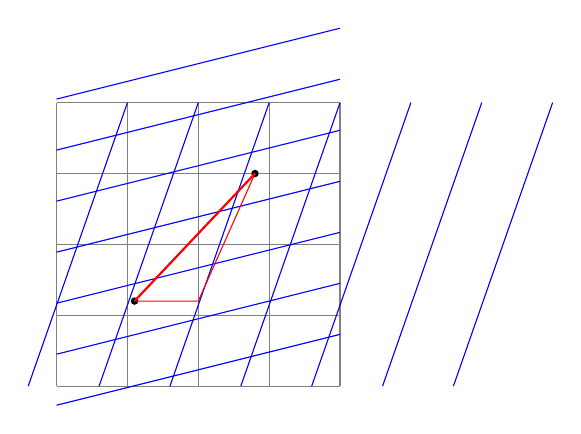
\begin{tikzpicture}[scale=0.9]
\draw[step=1,gray] (0,0) grid (4,4);

\foreach \k in {-1,0,1,2,3,4,5}
  \draw[blue] (\k+0.6,0) -- (\k+2.0,4);

\foreach \k in {-1,0,1,2,3,4,5}
  \draw[blue] (0,0.72*\k+0.45) -- (4,0.72*\k+1.45);

\fill (1.1,1.2) circle (1.5pt);
\fill (2.8,3.0) circle (1.5pt);
\draw[thick,red] (1.1,1.2) -- (2.8,3.0);
\draw[red] (1.1,1.2) -- (2.0,1.2) -- (2.8,3.0);
\end{tikzpicture}
\caption{Schematic redraw of the flat-plane picture: an orthogonal grid together with a skew coordinate net describing the same plane, and a highlighted interval whose Euclidean length is preserved.}
\end{figure}

Only after making these remarks about ordinary space does Susskind pivot to special relativity. A naive Euclidean guess in one time and one space dimension would be
\[
dt^2+dx^2.
\]
But this is not the quantity preserved by Lorentz transformations. The invariant interval is
\begin{equation}
d\tau^2=dt^2-dx^2.
\end{equation}
In three spatial dimensions,
\begin{equation}
d\tau^2=dt^2-dx^2-dy^2-dz^2.
\end{equation}

The lecture then pauses over units. Setting \(c=1\) is not just a convenience. It is the analog of measuring all spatial directions in the same units. If we insisted on measuring space and time in mismatched units, the formulas would be littered with conversion factors. In relativity, \(c\) is that conversion factor, and choosing \(c=1\) removes an artificial asymmetry.

Special relativity is then summarized in one line: it is the theory of coordinate transformations that preserve the form of this indefinite interval.

\section{General Space-Time Metric and the First Cosmological Example}

Now the lecture is ready to move from space to space-time. We switch from Latin to Greek indices and write the four coordinates as
\[
x^\mu,\qquad \mu=0,1,2,3,
\]
with \(x^0\) the time coordinate. This is the lecture's convention, and it is worth keeping because the notation itself helps mark the transition from spatial tensors to space-time tensors.

The natural generalization of the special-relativistic interval is exactly what the earlier tensor algebra suggests:
\begin{equation}
d\tau^2=g_{\mu\nu}(x)\,dx^\mu dx^\nu.
\end{equation}
At this stage one need not yet invoke genuine gravitation. One may already obtain nontrivial coordinate dependence by introducing curvilinear coordinates into flat space-time. The formalism comes first; the full gravitational interpretation comes later.

The flat special case is Minkowski space. In Minkowski coordinates the metric is
\begin{equation}
\eta_{\mu\nu}=\mathrm{diag}(1,-1,-1,-1),
\end{equation}
so that
\begin{equation}
d\tau^2=\eta_{\mu\nu}\,dx^\mu dx^\nu.
\end{equation}
The symbol \(\eta_{\mu\nu}\) is the space-time analog of \(\delta_{mn}\), except that its signature is not all plus. In the convention of this lecture there is one positive eigenvalue and three negative ones. Because the diagonal entries are \(\pm1\), the inverse is the same matrix:
\begin{equation}
\eta^{\mu\nu}=\eta_{\mu\nu}.
\end{equation}

The tensor rules themselves are unchanged. Contravariant objects still transform with \(\partial y/\partial x\), covariant ones with \(\partial x/\partial y\). The only novelty is the signature of the metric and the geometric meaning of the resulting scalar interval.

\subsection{Question \& Answer}

\paragraph{Question.} What does it mean, in the language of the metric, to say that space-time is expanding?

\paragraph{Answer.} It means that the metric coefficients depend on time in such a way that the spatial geometry changes with time. The lecture writes the diagonal matrix rather loosely, with entries \(1,-A(t),-A(t),-A(t)\), but describes the interval as having a squared scale factor. To match the interval as stated, the clean normalization is
\begin{equation}
d\tau^2=dt^2-a^2(t)\bigl(dx^2+dy^2+dz^2\bigr),
\end{equation}
where \(a(t)\) is the scale factor. If \(a(t)\) grows, then at fixed coordinate separations the spatial part of the metric grows, and that is what the lecture means here by an expanding universe.

Susskind then builds intuition by analogy rather than by curvature calculations. In two-dimensional space we already know
\begin{equation}
ds^2=dr^2+r^2 d\theta^2,
\end{equation}
which is just the plane written in polar coordinates. If we replace \(r^2\) by \(\sin^2 r\), we obtain
\begin{equation}
ds^2=dr^2+\sin^2 r\,d\theta^2,
\end{equation}
the metric of a sphere. If instead we take
\begin{equation}
ds^2=dr^2+e^{2r}d\theta^2,
\end{equation}
we obtain a horn-like surface whose circumference grows exponentially with \(r\).

The lecture's point is not yet to compute curvature. It is to teach us how to read geometry directly from metric coefficients. In the surface examples the geometry changes as a function of \(r\); in the cosmological example the geometry changes as a function of \(t\). That is the first concrete meaning of ``expanding space-time'' in the language of the metric tensor.

\section{Summary}

This lecture does two things at once. First, it completes the tensor algebra that general relativity cannot do without: transformation laws, mixed tensors, contraction, the metric, the inverse metric, and the raising and lowering of indices. Second, it uses exactly that machinery to pivot from ordinary space to space-time. Flat Euclidean geometry becomes Minkowski geometry, and Minkowski geometry becomes the general space-time line element
\[
d\tau^2=g_{\mu\nu}(x)\,dx^\mu dx^\nu.
\]
The lecture ends by postponing tensor calculus and curvature, but that postponement is itself part of the structure. We leave this chapter with the algebraic machinery in hand and with the first metric picture of an expanding universe already on the board.